% Figure 1: what the project does, in one picture.  Build: xelatex fig_overview.tex
\documentclass[border=1pt]{standalone}
\usepackage{fontspec}
\setmainfont{SourceSansPro-Regular.otf}[BoldFont=SourceSansPro-Semibold.otf, ItalicFont=SourceSansPro-RegularIt.otf]
\setmonofont{SourceCodePro-Regular.otf}[Scale=0.86]
\usepackage{amsmath}
\usepackage{tikz}
\usetikzlibrary{calc,arrows.meta}
\definecolor{ink}{HTML}{141413}
\definecolor{ink2}{HTML}{5E5D59}
\definecolor{ink3}{HTML}{87867F}
\definecolor{rule}{HTML}{DEDCD3}
\definecolor{ivory}{HTML}{F5F4EE}
\definecolor{clay}{HTML}{D97757}
\definecolor{clayl}{HTML}{F9ECE5}
\definecolor{blue}{HTML}{3F7CC0}
\newcommand{\cid}[1]{{\ttfamily #1}}
\newcommand{\g}[1]{\textcolor{ink2}{#1}}
\begin{document}
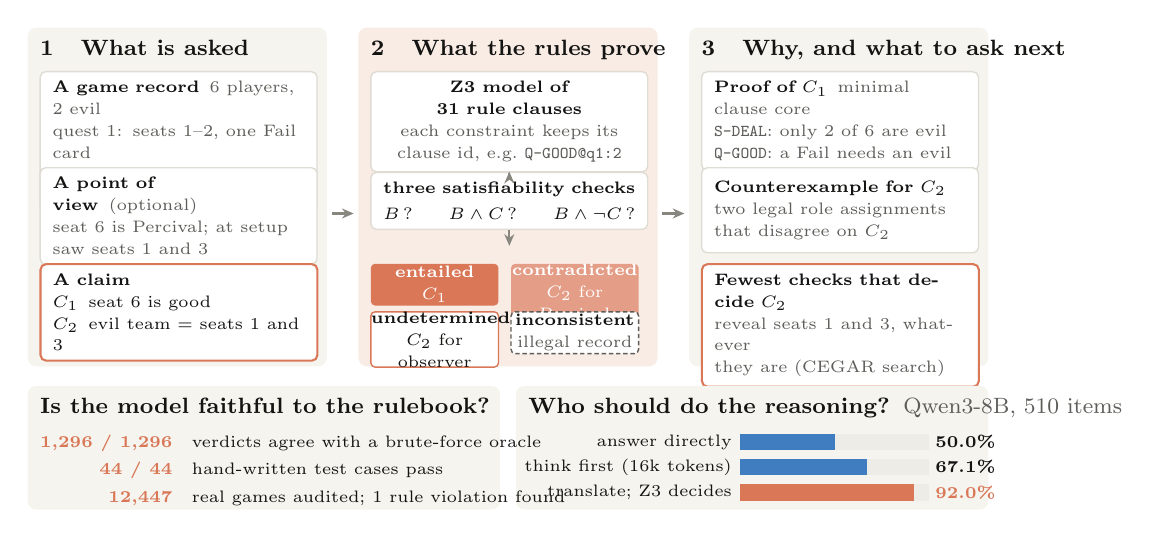
\begin{tikzpicture}[
  font=\fontsize{6.5}{7.9}\selectfont, color=ink, line width=0.5pt,
  % every card: one title line + two body lines, same height everywhere
  card/.style={draw=rule, fill=white, rounded corners=2pt, align=left, anchor=north west,
               inner xsep=4.5pt, inner ysep=3.5pt, text width=3.2cm, minimum height=1.08cm},
  head/.style={font=\fontsize{7.8}{9}\selectfont\bfseries, anchor=north west, inner sep=0pt},
  arr/.style={-{Stealth[length=4.2pt,width=3.6pt]}, color=ink3, line width=0.75pt},
  chip/.style={rounded corners=1.5pt, minimum height=0.53cm, text width=1.62cm, align=center, inner sep=0pt,
               anchor=north west},
]
% ================================================================ panels: 3 x 3.80 cm, gaps 0.40 cm
\fill[ivory, rounded corners=3pt] (0.00,0) rectangle (3.80,-4.30);
\fill[clayl, rounded corners=3pt] (4.20,0) rectangle (8.00,-4.30);
\fill[ivory, rounded corners=3pt] (8.40,0) rectangle (12.20,-4.30);
\node[head] at (0.15,-0.15) {1\quad What is asked};
\node[head] at (4.35,-0.15) {2\quad What the rules prove};
\node[head] at (8.55,-0.15) {3\quad Why, and what to ask next};
\draw[arr] (3.86,-2.36) -- (4.14,-2.36);
\draw[arr] (8.06,-2.36) -- (8.34,-2.36);

% ================================================================ 1: the question (rows at -0.55, -1.77, -2.99)
\node[card] at (0.15,-0.55) {\textbf{A game record}\enspace\g{6 players, 2 evil}\\
  \g{quest 1: seats 1--2, one Fail card}\\ \g{quest 2: seats 3--5, one Fail card}};
\node[card] at (0.15,-1.77) {\textbf{A point of view}\enspace\g{(optional)}\\
  \g{seat 6 is Percival; at setup}\\ \g{saw seats 1 and 3}};
\node[card, draw=clay, line width=0.75pt] at (0.15,-2.99) {\textbf{A claim}\\
  $C_1$\enspace seat 6 is good\\ $C_2$\enspace evil team = seats 1 and 3};

% ================================================================ 2: the verifier
\node[card, align=center] (enc) at (4.35,-0.55) {\textbf{Z3 model of 31 rule clauses}\\
  \g{each constraint keeps its}\\ \g{clause id, e.g.\ \cid{Q-GOOD@q1:2}}};
\node[card, align=center, minimum height=0.72cm] (chk) at (4.35,-1.83) {\textbf{three satisfiability checks}\\[1.5pt]
  $B$\,?\quad\; $B\wedge C$\,?\quad\; $B\wedge\neg C$\,?};
\draw[arr] (enc.south) -- (chk.north);
\draw[arr] (chk.south) -- ++(0,-0.20);
\node[chip, fill=clay, text=white]                               at (4.35,-2.99) {\textbf{entailed}\\ $C_1$};
\node[chip, fill=clay!72!white, text=white]                      at (6.13,-2.99) {\textbf{contradicted}\\ $C_2$ for Percival};
\node[chip, fill=white, draw=clay]                               at (4.35,-3.60) {\textbf{undetermined}\\ $C_2$ for observer};
\node[chip, fill=white, draw=ink2, dash pattern=on 1.6pt off 1pt] at (6.13,-3.60) {\textbf{inconsistent}\\ \g{illegal record}};

% ================================================================ 3: evidence and the next question
\node[card] at (8.55,-0.55) {\textbf{Proof of $C_1$}\enspace\g{minimal clause core}\\
  \g{\cid{S-DEAL}: only 2 of 6 are evil}\\ \g{\cid{Q-GOOD}: a Fail needs an evil}};
\node[card] at (8.55,-1.77) {\textbf{Counterexample for $C_2$}\\
  \g{two legal role assignments}\\ \g{that disagree on $C_2$}};
\node[card, draw=clay, line width=0.75pt] at (8.55,-2.99) {\textbf{Fewest checks that decide $C_2$}\\
  \g{reveal seats 1 and 3, whatever}\\ \g{they are (CEGAR search)}};

% ================================================================ bottom strip: two findings
\fill[ivory, rounded corners=3pt] (0.00,-4.55) rectangle (6.00,-6.12);
\fill[ivory, rounded corners=3pt] (6.20,-4.55) rectangle (12.20,-6.12);
\node[head] at (0.15,-4.70) {Is the model faithful to the rulebook?};
\node[anchor=north west, inner sep=0pt] at (0.15,-5.08) {%
  \renewcommand{\arraystretch}{1.25}%
  \begin{tabular}{@{}r@{\hspace{7pt}}l@{}}
  \textcolor{clay}{\bfseries 1,296 / 1,296} & verdicts agree with a brute-force oracle\\
  \textcolor{clay}{\bfseries 44 / 44} & hand-written test cases pass\\
  \textcolor{clay}{\bfseries 12,447} & real games audited; 1 rule violation found
  \end{tabular}};
\node[head] at (6.35,-4.70) {Who should do the reasoning?\enspace\g{\mdseries Qwen3-8B, 510 items}};
% bars: labels end at 8.95, track 9.05 -- 11.45, values at 11.52
\foreach \y/\t in {-5.26/answer directly, -5.58/think first (16k tokens), -5.90/translate; Z3 decides}
  {\node[anchor=east, inner sep=0pt] at (8.95,\y) {\t};
   \fill[rule!55!white] (9.05,\y-0.105) rectangle (11.45,\y+0.105);}
\fill[blue] (9.05,-5.365) rectangle (10.250,-5.155);
\fill[blue] (9.05,-5.685) rectangle (10.660,-5.475);
\fill[clay] (9.05,-6.005) rectangle (11.258,-5.795);
\node[anchor=west, inner sep=0pt, font=\fontsize{6.5}{7.9}\selectfont\bfseries] at (11.52,-5.26) {50.0\%};
\node[anchor=west, inner sep=0pt, font=\fontsize{6.5}{7.9}\selectfont\bfseries] at (11.52,-5.58) {67.1\%};
\node[anchor=west, inner sep=0pt, font=\fontsize{6.5}{7.9}\selectfont\bfseries, color=clay] at (11.52,-5.90) {92.0\%};
\end{tikzpicture}
\end{document}
